\section{Training operators to assemble a starter motor}\label{sec:training}

Small parts assembly of flexible components is a very challenging task to automate given the advanced sensing and gripping technologies that it requires. As such, currently it is more cost effective to have cooperative assembly lines in which humans perform the tasks that require robust perception, adaptive grasping and high level cognition while the robot does the remaining tasks.

In the next sections we will present the application of our immersive training system for the assembly of a starter motor. This is a representative use case of small parts assembly given its diversity of operations and components. Moreover, since it has flexible parts (rubbers, wires, springs), it would be a prime candidate for a collaborative assembly line, in which besides teaching, our immersive \gls{hmi} system could also be used to coordinate the assembly process between the operator and the robotic system.



\subsection{Testing platform}

Our immersive teaching system was developed as a \gls{ros} Kinetic\footnote{\url{http://www.ros.org}} package for fast integration into robotic systems and relies on the Gazebo simulator for 3D rendering and the \gls{pcl} for 3D perception. It was tested with a BenQ W1070 \gls{dlp} projector\footnote{\url{http://www.benq.com/product/projector/W1070}} for projecting the teaching information, an Asus Xtion Pro Live\footnote{\url{https://www.asus.com/3D-Sensor/Xtion_PRO_LIVE}} structured light 3D sensor for object recognition and a Kinect 2\footnote{\url{http://www.xbox.com/en-US/xbox-one/accessories/kinect}} \gls{tof} 3D sensor for the user interaction analysis. In \cref{fig:hardware} it can be seen the work area and the hardware disposition (in the right image the projector is on the top right, the Kinect 2 is on the left, the Asus Xtion is below the projector and the David Laser 3D structured light system camera is at the top).

\begin{figure}[H]
	\centering
	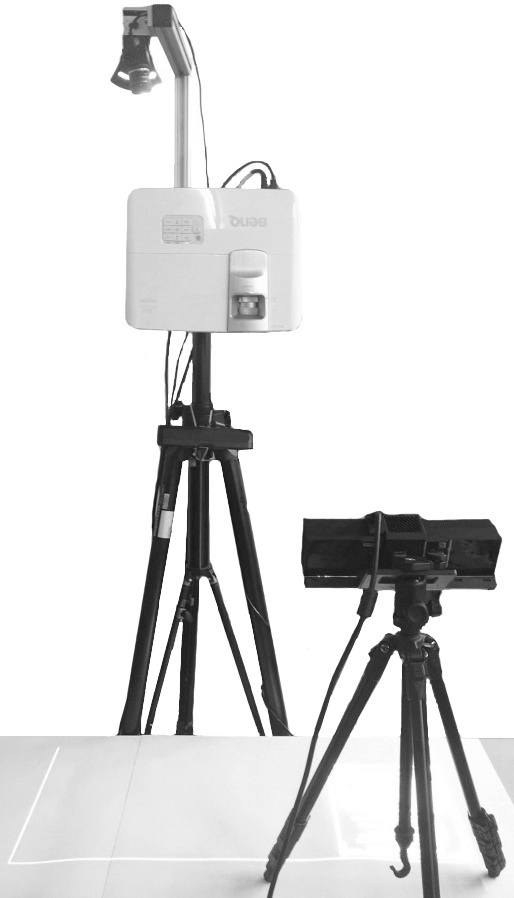
\includegraphics[height=.26\textheight]{hardware-front}
	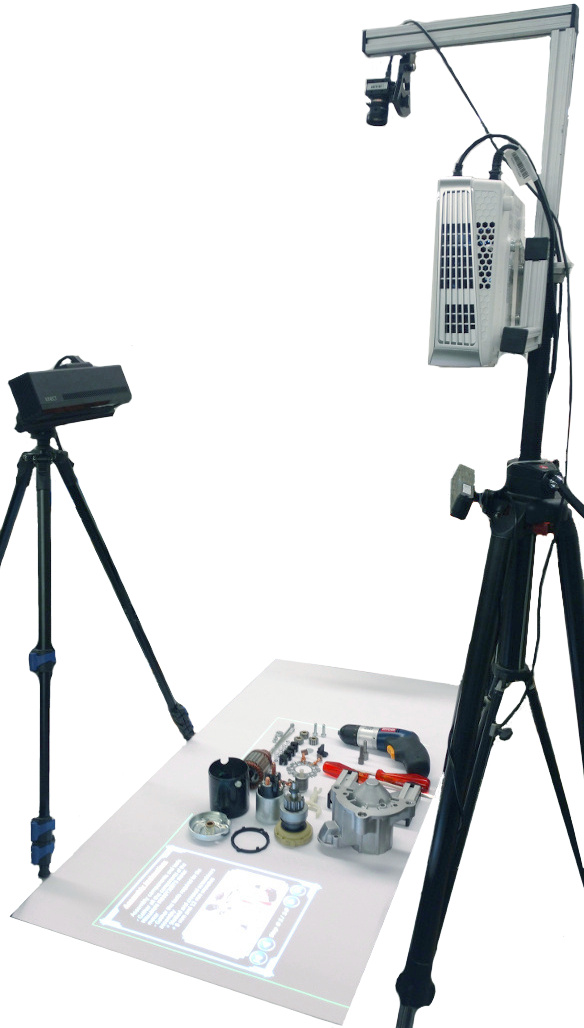
\includegraphics[height=.26\textheight]{hardware-side}
	\caption{Hardware setup}
	\label{fig:hardware}
\end{figure}


\subsection{Training session}

The training session started by gathering all the assembly parts and the required tools for performing the starter motor assembly (shown in \cref{fig:assembly-parts}). Then using the immersive teaching system, the operator read the instructions, watched the videos and navigated through the assembly steps using the projected interaction buttons (presented in \cref{fig:interaction-pause,fig:interaction-seek,fig:interaction-first-0,fig:interaction-first-1}) until it completed the assembly process (starter motor after assembly shown in \cref{fig:projection-mapping-1,fig:projection-mapping-2}). In the last assembly step the projection mapping system projected the outline of the expected starter motor geometry to help the operator perform a visual inspection in order to make sure that the final assembled object was mounted correctly (example of the validation projection in \cref{fig:projection-mapping-1,fig:projection-mapping-2}). During this last step, the object recognition system detected and tracked the final assembled product while also updating the virtual 3D model in order to accurately render and project the outline of the starter engine into the workspace.


\begin{figure}[ht!]
	\begin{floatrow}[2]
		\ffigbox[\FBwidth]
		{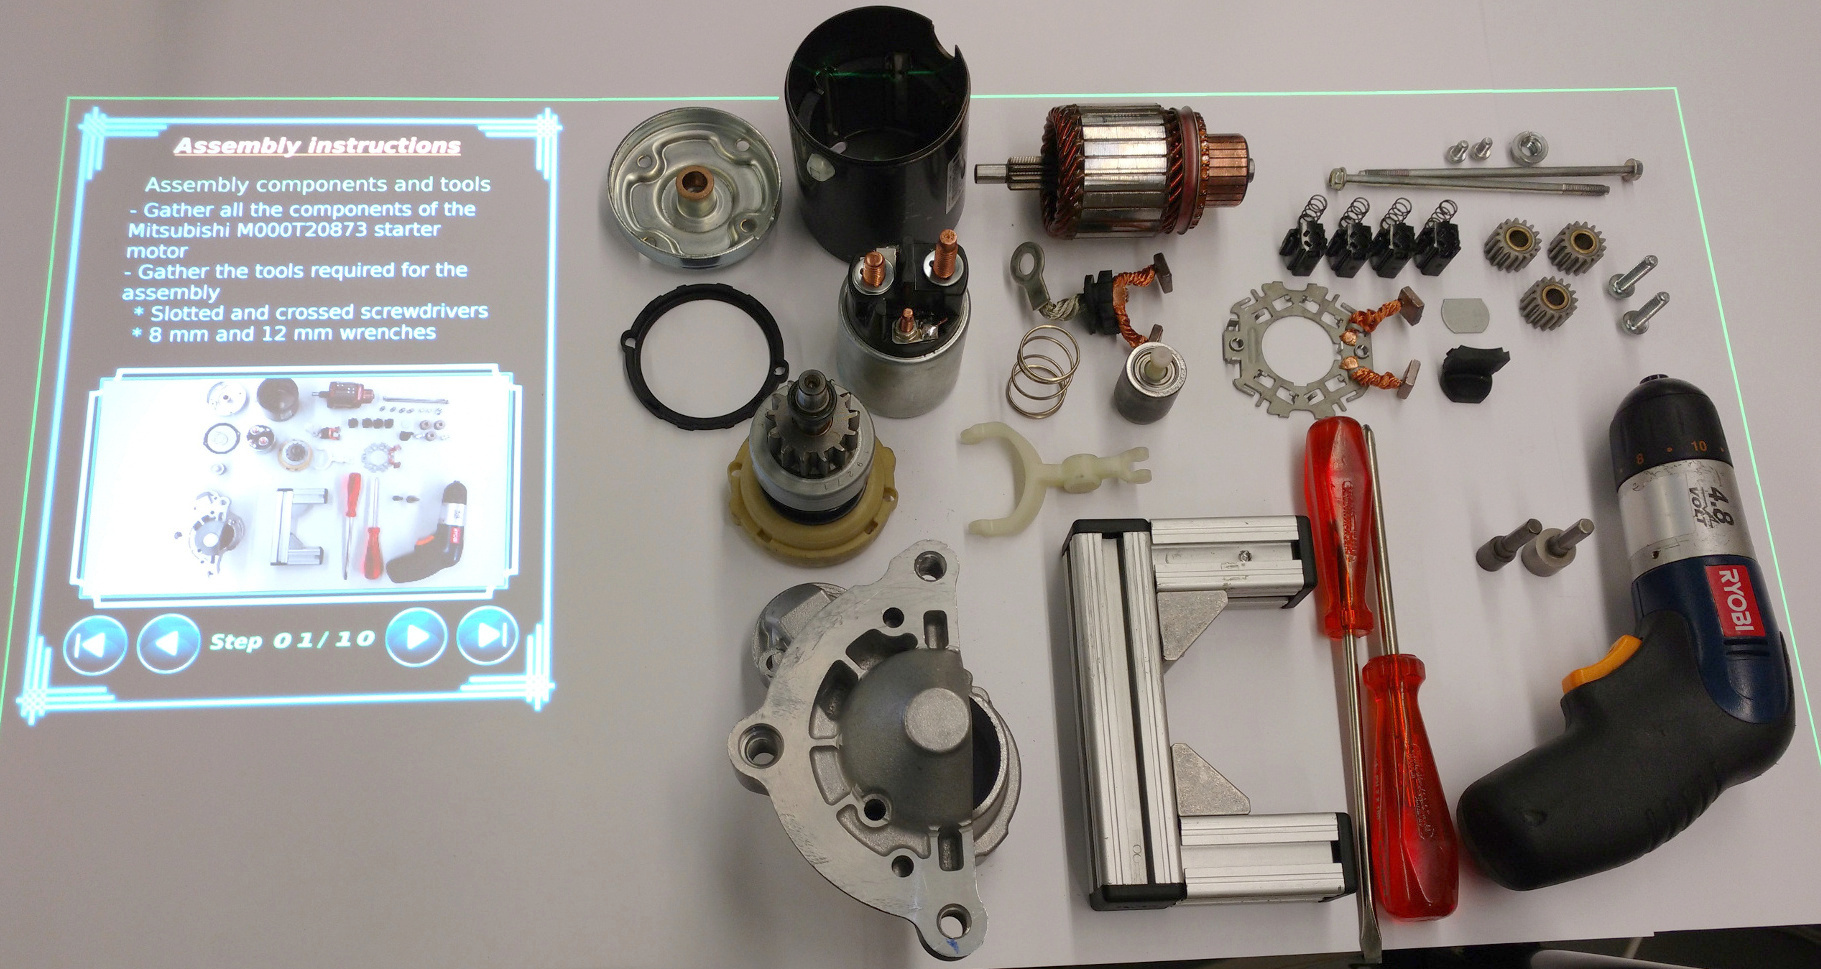
\includegraphics[height=.175\textheight]{assembly-parts}}
		{\caption{Starter motor parts and assembly tools}\label{fig:assembly-parts}}
		\ffigbox[\FBwidth]
		{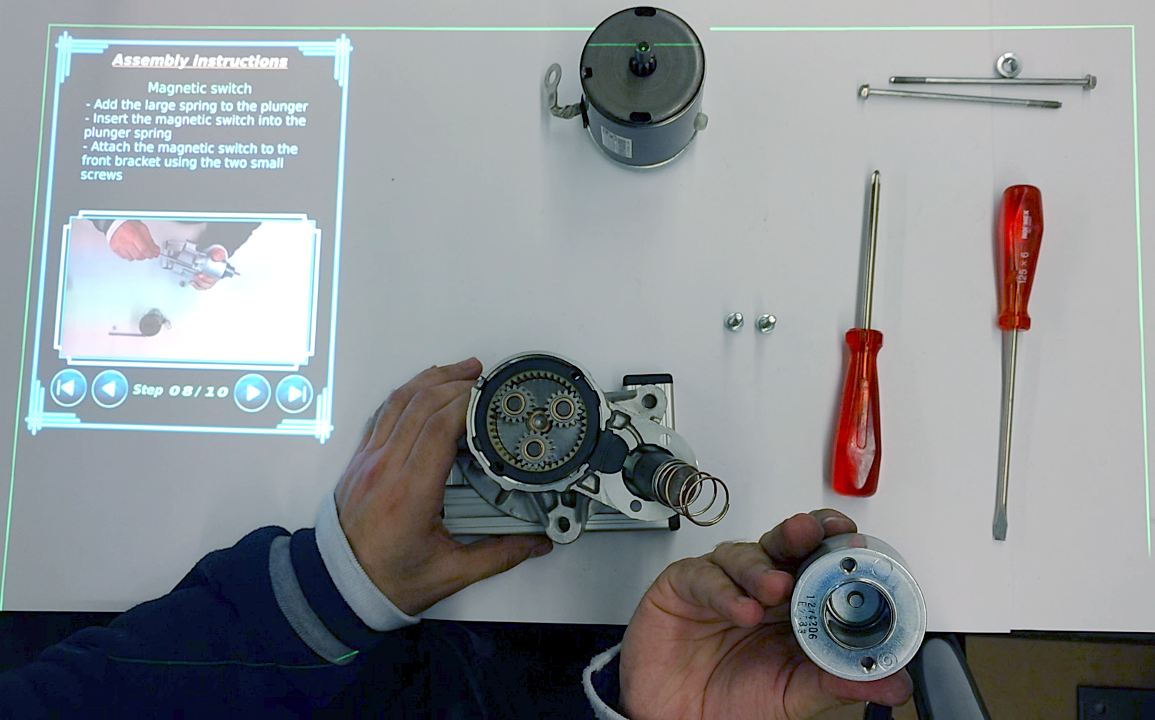
\includegraphics[height=.175\textheight]{assembly}}
		{\caption{Operator assembling starter motor}\label{fig:assembly}}
	\end{floatrow}
\end{figure}

\begin{figure}[ht!]
	\begin{floatrow}[2]
		\ffigbox[\FBwidth]
		{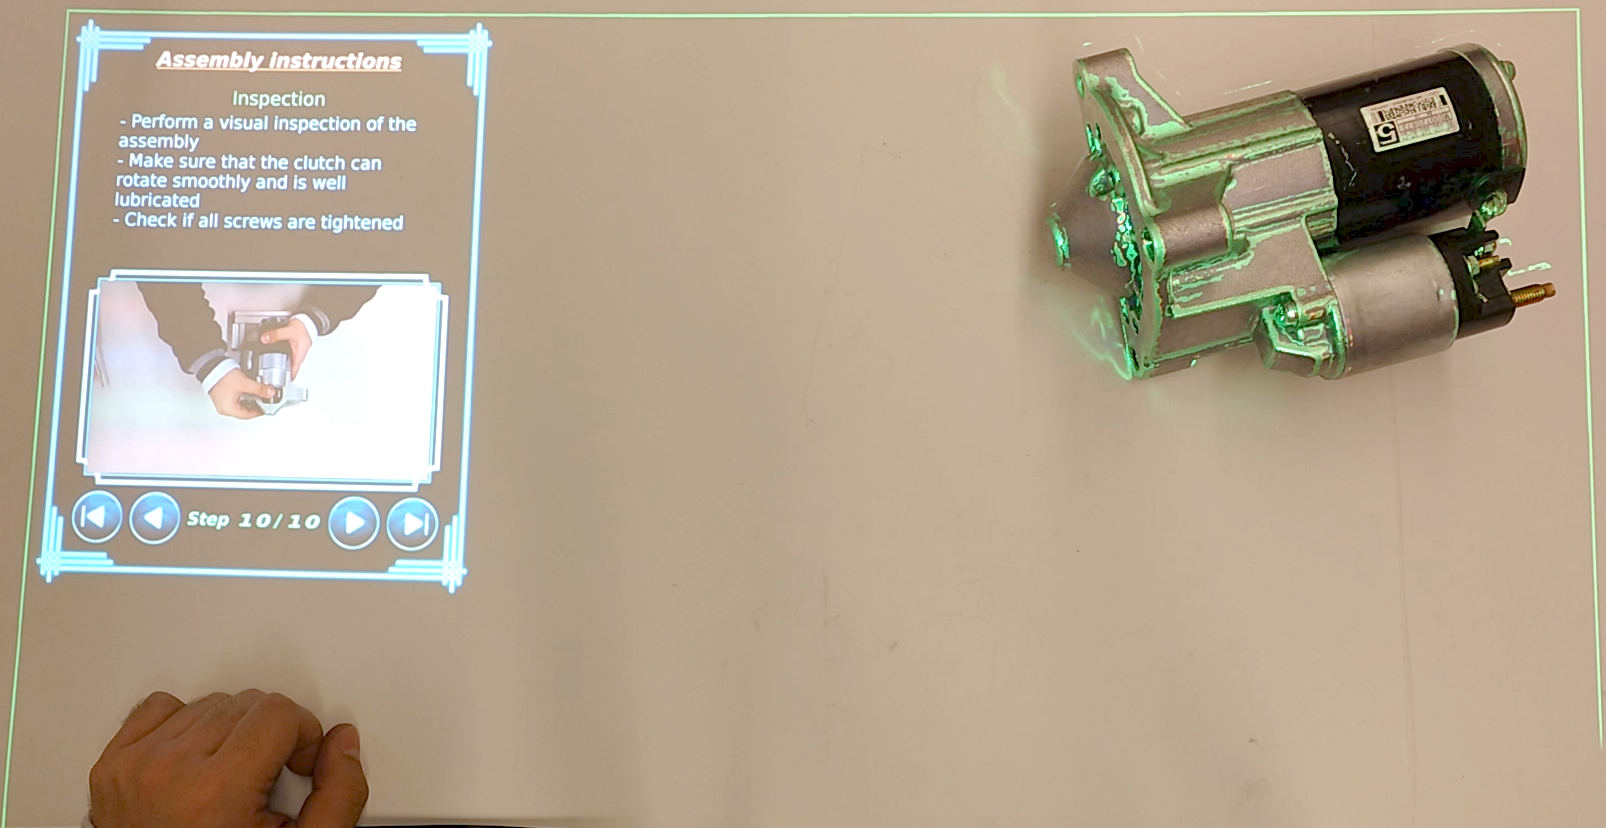
\includegraphics[height=.187\textheight]{projection-mapping-1}}
		{\caption{Projection of the reconstructed 3D model (texture colorized using the surface normal curvature information)}\label{fig:projection-mapping-1}}
		\ffigbox[\FBwidth]
		{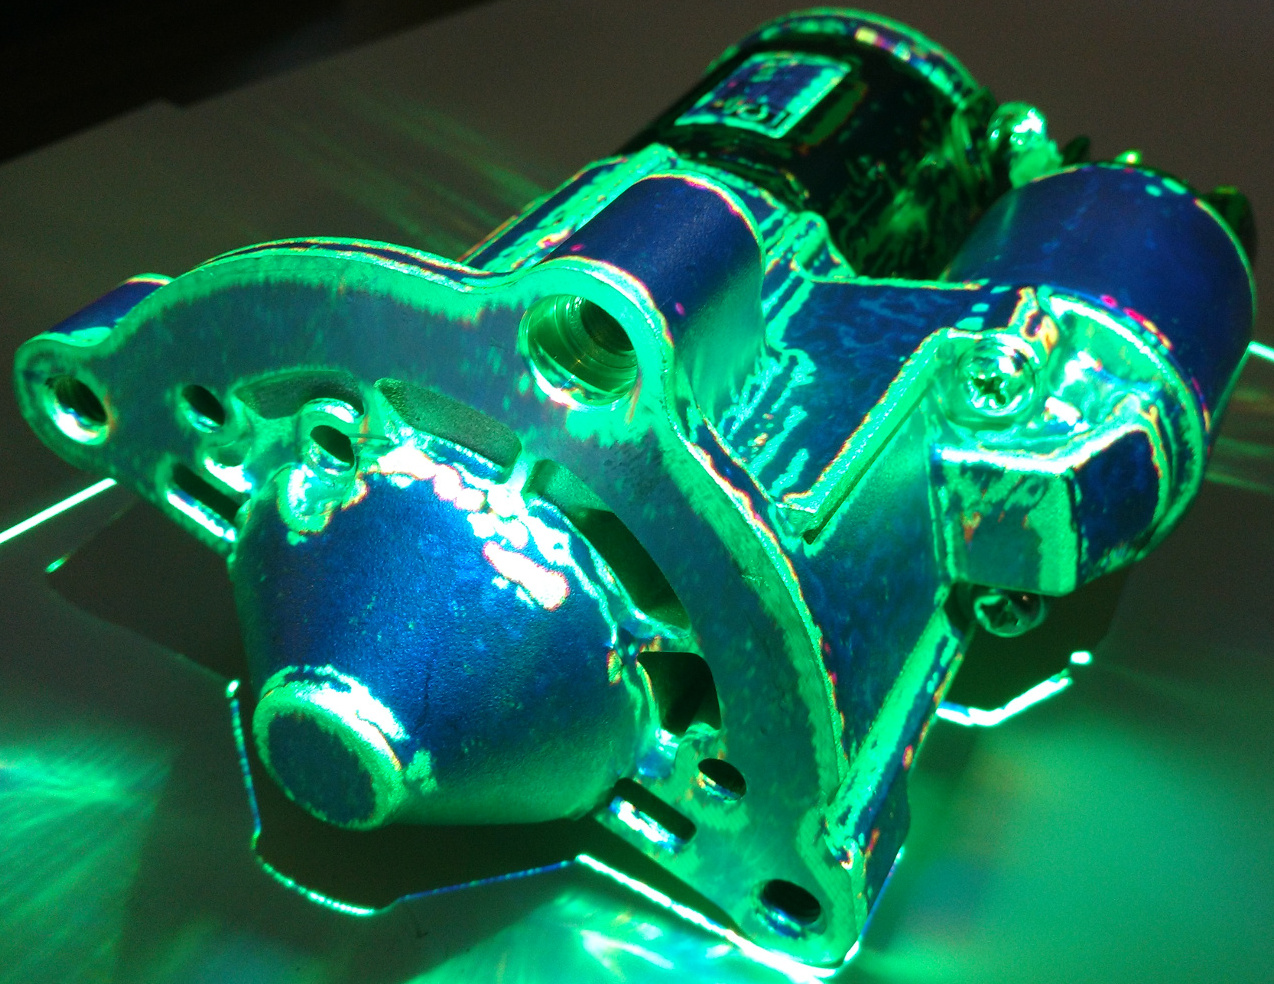
\includegraphics[height=.187\textheight]{projection-mapping-3}}
		{\caption{Detailed view of the assembled object validation projection}\label{fig:projection-mapping-2}}
	\end{floatrow}
\end{figure}

\begin{figure}[ht!]
	\begin{floatrow}[4]
		\ffigbox[\FBwidth]
		{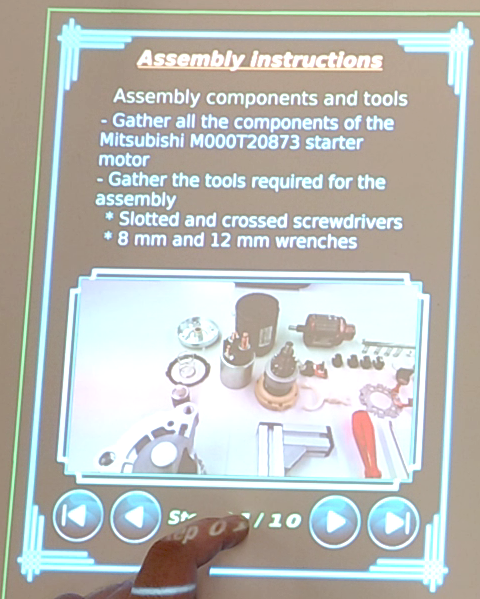
\includegraphics[height=.177\textheight]{interaction-pause}}
		{\caption{Example of video play / pause interaction}\label{fig:interaction-pause}}
		\ffigbox[\FBwidth]
		{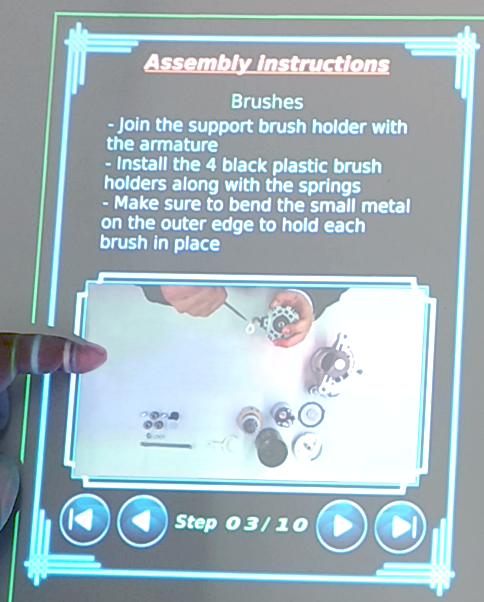
\includegraphics[height=.177\textheight]{interaction-seek}}
		{\caption{Example of video seek interaction}\label{fig:interaction-seek}}
		\ffigbox[\FBwidth]
		{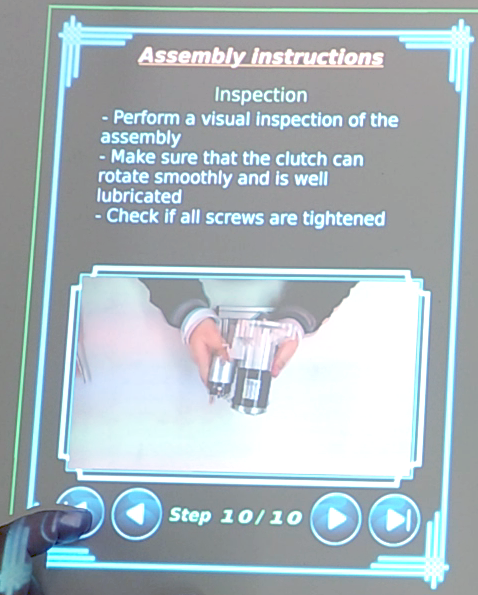
\includegraphics[height=.177\textheight]{interaction-first-0}}
		{\caption{Example of request move to the first step}\label{fig:interaction-first-0}}
		\ffigbox[\FBwidth]
		{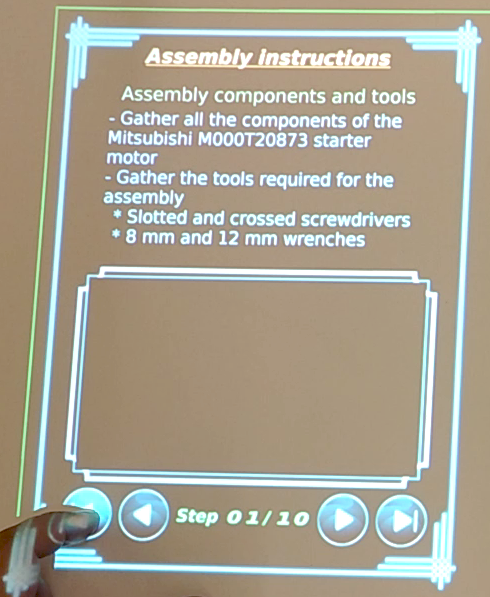
\includegraphics[height=.177\textheight]{interaction-first-1}}
		{\caption{Visual feedback for button action}\label{fig:interaction-first-1}}
	\end{floatrow}
\end{figure}
